\begin{figure}
        \centering
\pgfplotsset{every axis/.append style={semithick}, legend style={nodes={scale=0.7, transform shape}, at={(1,0)},anchor=south east}}
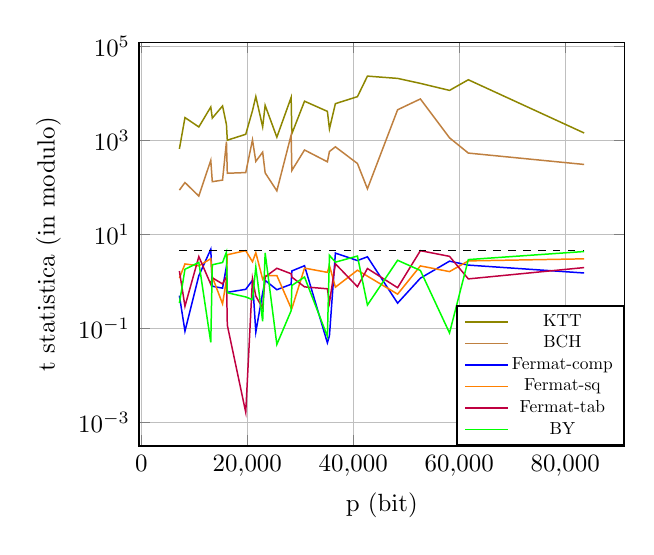
\begin{tikzpicture}[scale=0.9]
	\begin{semilogyaxis}[
        xlabel=p (bit),ylabel=t statistica (in modulo), grid=major, xticklabel style={
            /pgf/number format/fixed,
            /pgf/number format/precision=5
            }, scaled x ticks=false ]

        \addplot[no marks, color=olive] coordinates {
            (7187, 652.005696)
            (8237, 3019.920377)
            (10853, 1910.771944)
            (13109, 5071.778073)
            (13397, 2946.893161)
            (15331, 5332.226134)
            (16067, 2139.75731)
            (16229, 998.246284)
            (19709, 1332.526004)
            (20981, 4239.90178)
            (21611, 8454.250835)
            (22901, 1920.498214)
            (23371, 5492.804618)
            (25579, 1155.64429)
            (28277, 8096.484658)
            (28411, 1371.076919)
            (30803, 6732.774469)
            (35117, 4094.864009)
            (35507, 1734.952881)
            (36629, 5973.390682)
            (40787, 8408.629239)
            (42677, 23009.76453)
            (48371, 20572.562632)
            (52667, 16117.718704)
            (58171, 11429.139155)
            (61717, 19250.383818)
            (83579, 1419.418492)
    };
    \addlegendentry{KTT}
    
    \addplot[no marks, color=brown] coordinates {
            (7187, 86.646338)
            (8237, 125.408114)
            (10853, 64.681601)
            (13109, 372.819976)
            (13397, 130.796415)
            (15331, 141.441714)
            (16067, 928.621171)
            (16229, 197.779837)
            (19709, 204.312264)
            (20981, 1011.501825)
            (21611, 353.268775)
            (22901, 554.996088)
            (23371, 201.444914)
            (25579, 83.641382)
            (28277, 1285.511342)
            (28411, 226.541613)
            (30803, 617.673131)
            (35117, 346.507444)
            (35507, 573.58292)
            (36629, 720.523447)
            (40787, 318.858938)
            (42677, 92.41314)
            (48371, 4425.944718)
            (52667, 7515.104843)
            (58171, 1120.57332)
            (61717, 531.092093)
            (83579, 304.239061)
    };
    \addlegendentry{BCH}
    
    \addplot[no marks, color=blue] coordinates {
            (7187, 0.493086)
            (8237, 0.08653)
            (10853, 1.309049)
            (13109, 4.778504)
            (13397, 0.782128)
            (15331, 0.71157)
            (16067, 2.079124)
            (16229, 0.580534)
            (19709, 0.672241)
            (20981, 1.0493)
            (21611, 0.083094)
            (22901, 0.567385)
            (23371, 1.04121)
            (25579, 0.660099)
            (28277, 0.861794)
            (28411, 1.653982)
            (30803, 2.134661)
            (35117, 0.048959)
            (35507, 0.06948)
            (36629, 3.96631)
            (40787, 2.752093)
            (42677, 3.304725)
            (48371, 0.341822)
            (52667, 1.160096)
            (58171, 2.671217)
            (61717, 2.201135)
            (83579, 1.496464)
    };
    \addlegendentry{Fermat-comp}
    
    \addplot[no marks, color=orange] coordinates {
            (7187, 1.162409)
            (8237, 2.330743)
            (10853, 2.12729)
            (13109, 3.016198)
            (13397, 1.238996)
            (15331, 0.330162)
            (16067, 1.078995)
            (16229, 3.658359)
            (19709, 4.467738)
            (20981, 2.591605)
            (21611, 4.04695)
            (22901, 1.106657)
            (23371, 1.312441)
            (25579, 1.322171)
            (28277, 0.266311)
            (28411, 0.262227)
            (30803, 1.901191)
            (35117, 1.544098)
            (35507, 2.154404)
            (36629, 0.747209)
            (40787, 1.713264)
            (42677, 1.281831)
            (48371, 0.530638)
            (52667, 2.117118)
            (58171, 1.600775)
            (61717, 2.704511)
            (83579, 2.992715)
    };
    \addlegendentry{Fermat-sq}
    
    \addplot[no marks, color=purple] coordinates {
            (7187, 1.646462)
            (8237, 0.293479)
            (10853, 3.342243)
            (13109, 0.860273)
            (13397, 1.182994)
            (15331, 0.875522)
            (16067, 1.25272)
            (16229, 0.116413)
            (19709, 0.001627)
            (20981, 1.131281)
            (21611, 0.481985)
            (22901, 0.268159)
            (23371, 1.231348)
            (25579, 1.886799)
            (28277, 1.441204)
            (28411, 1.222019)
            (30803, 0.758732)
            (35117, 0.690352)
            (35507, 0.351563)
            (36629, 2.346714)
            (40787, 0.764265)
            (42677, 1.863431)
            (48371, 0.727855)
            (52667, 4.463352)
            (58171, 3.378872)
            (61717, 1.119912)
            (83579, 1.95091)
    };
    \addlegendentry{Fermat-tab}
    
    \addplot[no marks, color=green] coordinates {
            (7187, 0.342964)
            (8237, 1.79303)
            (10853, 2.511967)
            (13109, 0.05001)
            (13397, 2.238948)
            (15331, 2.499593)
            (16067, 4.175354)
            (16229, 0.568396)
            (19709, 0.462919)
            (20981, 0.405652)
            (21611, 2.010867)
            (22901, 0.140311)
            (23371, 4.014809)
            (25579, 0.045285)
            (28277, 0.236084)
            (28411, 0.81202)
            (30803, 1.22736)
            (35117, 0.06737)
            (35507, 3.550464)
            (36629, 2.543941)
            (40787, 3.429449)
            (42677, 0.312068)
            (48371, 2.789529)
            (52667, 1.693412)
            (58171, 0.0794)
            (61717, 2.885019)
            (83579, 4.281391)
    };
    \addlegendentry{BY}

    \addplot[no marks, color=black, style=dashed] coordinates {
        (7187, 4.5)
        (83579, 4.5)
    };
    

    \end{semilogyaxis}%
\end{tikzpicture}%
\caption{Valori della t di Student}
\end{figure}